\documentclass[aps,onecolumn]{revtex4}
\usepackage{graphicx}
\usepackage{amssymb,amsfonts,amsmath,amsthm}
\usepackage{chemarr}
\usepackage{bm}
\usepackage{pslatex}
\usepackage{mathptmx}
\usepackage{xfrac}
\usepackage{xcolor}

\begin{document}

\section{Curvature of a revolution surface}

\begin{equation}
	\vec{M}(u,v) = 
	\begin{bmatrix}
	r(u)\cos v\\
	r(u)\sin v\\
	z(u)
	\end{bmatrix},
	\;\;
	\vec{M}_u = 
	\begin{bmatrix}
	\dot{r}\cos v\\
	\dot{r}\sin v\\
	\dot{z}
	\end{bmatrix},
	\;\;
	\vec{M}_v = 
	\begin{bmatrix}
	-r \sin v\\
	 r \cos v\\
	 0
	\end{bmatrix},
	\;\;
	\vec{M}_{uu} = 
	\begin{bmatrix}
	\ddot{r} \cos v\\
	\ddot{r} \sin v\\
	\ddot{z}
	\end{bmatrix},
	\;\;
	\vec{M}_{vv} = 
	\begin{bmatrix}
	-r \cos v\\
	-r \sin v\\
	0
	\end{bmatrix},
	\;\;
	\vec{M}_{uv} = 
	\begin{bmatrix}
	-\dot{r} \sin v\\
	 \dot{r} \cos v\\
	 0
	\end{bmatrix}
\end{equation}

\begin{equation}
	E = \vec{M}_u^2 = \dot{r}^2 + \dot{z}^2,\;\;
	F = \vec{M}_u \cdot \vec{M}_v = 0,\;\;
	G = \vec{M}_v^2 = r^2
\end{equation}

\begin{equation}
	\vec{n} = \vec{M}_u \wedge \vec{M}_v = 
	\begin{bmatrix}
	-r\dot{z}\cos v\\
	-r\dot{z}\sin v\\
	r\dot{r}
	\end{bmatrix},\;\;
	\left\vert\vec{M}_u \wedge \vec{M}_v\right\vert = r\left(\dot{r}^2 + \dot{z}^2\right)^{1/2}
\end{equation}

\begin{equation}
	L = \vec{n}\cdot\vec{M}_{uu} = r\left(\dot{r}\ddot{z}-\dot{z}\ddot{r}\right),\;\;
	M = \vec{n}\cdot\vec{M}_{uv} = 0,
	\;\;
	N = \vec{n}\cdot\vec{M}_{vv} = r^2\dot{z}
\end{equation}

Then
\begin{equation}
	EN + GL - 2FM = r^2 \dot{z} \left(\dot{r}^2 + \dot{z}^2\right) + r^3\left(\dot{r}\ddot{z}-\dot{z}\ddot{r}\right)
\end{equation}
and
\begin{equation}
	EG - F^2 = r^2 \left(\dot{r}^2 + \dot{z}^2\right).
\end{equation}
Finally, 
\begin{equation}
	\mathcal{H} = \dfrac{1}{2\left\vert\vec{n}\right\vert} \dfrac{EN + GL - 2FM}{EG - F^2} =
	\dfrac{\dot{z} \left(\dot{r}^2 + \dot{z}^2\right) + r\left(\dot{r}\ddot{z}-\dot{z}\ddot{r}\right)}
	{2r\left(\dot{r}^2 + \dot{z}^2\right)^{3/2}}
\end{equation}

\section{Using a curvilinear profile}
We now use an intrinsic representation of the $(r,z)$ profile using the
angle $\phi$ and the variable $s$ so that
\begin{equation}
\left\lbrace
	\begin{array}{rcl}
	r' & = & \cos \phi\\
	z' & = & \sin \phi\\
	r'' & = & -\sin\phi \phi'\\
	z'' & = & \cos\phi  \phi'\\
	\end{array}
\right.
\end{equation}
and we get
\begin{equation}
	\mathcal{H} = \frac{1}{2} \left(\phi'+\dfrac{\sin\phi}{r}\right)
\end{equation}

\section{Surface equation}
\subsection{Real Units}
Since the capillary pressure is supporting the liquid
\begin{equation}
	\gamma \mathcal{H} = \rho g z
\end{equation}
or using the capillary length
\begin{equation}
	\lambda = \sqrt{\dfrac{\gamma}{\rho g}}
\end{equation}

\begin{equation}
	\mathcal{H} = \dfrac{z}{\lambda^2}
\end{equation}
leading to
\begin{equation}
	\partial_s \phi = \dfrac{z}{2\lambda^2} - \dfrac{\sin\phi}{r}
\end{equation}

\subsection{Reduced units}
We rescale w.r.t the apex radius $R_0$ using
\begin{equation}
	\left\lbrace
	\begin{array}{rcl}
		\tau & = & s/R_0 \\
		 u   & = & r/R_0 \\
		 v   & = & z/R_0 \\
	\end{array}
	\right.
\end{equation}
to get
\begin{equation}
	\left\lbrace
	\begin{array}{rcl}
	\partial_\tau u & = & \cos\phi\\
	\partial_\tau v & = & \sin\phi\\
	\partial_\tau \phi & = &  \mu^2 v - \dfrac{\sin\phi}{u}\\
	\\
	\zeta              & = & \dfrac{h}{R_0}\\
	\\
	\mu                & = & \dfrac{R_0^2}{2\lambda^2}\\
	\end{array}
	\right.
\end{equation}
	
\subsection{Initial conditions}

\begin{center}
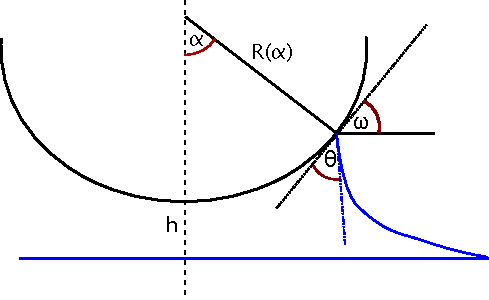
\includegraphics{geometry.pdf}
\end{center}

For a given $(\theta,\alpha)$, the initial coordinates are
\begin{equation}
\left\lbrace
\begin{array}{rcl}
	r_0    & = & R(\alpha) \sin(\alpha)\\
	z_0    & = & (h + R_0) - R(\alpha) \cos(\alpha)\\
	\phi_0 & = & \left(\omega + \theta\right) - \pi\\
\end{array}
\right. 
\end{equation}
where $\omega$ is $\alpha$ for a sphere.\\
We hence get
\begin{equation}
\left\lbrace
\begin{array}{rcl}
	u_0    & = & \sin\alpha\\
	v_0    & = & \zeta + (1-\cos\alpha)\\
	\phi_0 & = & \alpha+\theta-\pi\\
\end{array}
\right.
\end{equation}

%Valid initial conditions are defined by
%\begin{itemize}
%\item $r>0$, which excludes starting at $\alpha=0$ or $\alpha=\pi$.
%\item ...
%\end{itemize}
%
%\subsubsection{Numerical Integration}
%During integration, a guest $(r,z)$ is found.
%We have some 'failure' cases
%\begin{itemize}
%\item $r\leq0$
%\item $(r,z)$ re-entered the lens...
%\end{itemize}
%
%The we have some normal stop conditions
%\begin{itemize}
%\item $\partial_s r = \cos \phi$ is positive and become negative.
%\item $\partial_s z = \sin \phi$ changes its sign.
%\end{itemize}
%
%Let us start from

\end{document}